\subsection*{Основные теоремы}

{

\begin{wrapfigure}{o}{27mm}
\vskip-5mm
\centering
\includegraphics{mppics/ris-extra-3}
\caption{}\label{extra/ris-3}
\end{wrapfigure}

\paragraph{}\label{1938/70}
\mbox{\so{Определение}.}
Две прямые называются \rindex{параллельные прямые}\textbf{параллельными}, если они лежат в одной плоскости и \textbf{не пересекаются}, сколько бы их ни продолжали.
При этом прямая также считается параллельной самой себе.


Параллельность прямых обозначается письменно знаком $\parallel$.
Так, если прямые $AB$ и $CD$ параллельны, то пишут:
$AB \parallel CD$. 
На чертежах параллельные прямые принято отмечать одинаковыми стрелочками как на рис. \ref{extra/ris-3}.

Существование параллельных прямых обнаруживается следующей теоремой.

}

\paragraph{}\label{1938/71}
\mbox{\so{Теорема}.}
\textbf{\emph{Два перпендикуляра}} ($AB$ и $CD$, рис.~\ref{1938/ris-72}) \textbf{\emph{к одной и той же прямой}} ($MN$) \textbf{\emph{не могут пересечься, сколько бы мы их ни продолжали.}}

\begin{wrapfigure}[11]{o}{34mm}
\vskip-0mm
\centering
\includegraphics{mppics/ris-72}
\caption{}\label{1938/ris-72}
\end{wrapfigure}

Действительно, если бы эти перпендикуляры пересеклись в какой-нибудь точке $P$, то из этой точки на прямую $MN$ были бы опущены два перпендикуляра, что невозможно (§~\ref{1938/24}).
Таким образом, \emph{два перпендикуляра к одной прямой параллельны между собой.}

\paragraph{Названия углов, получаемых при пересечении двух прямых третьей.}\label{1938/72}
Пусть две прямые $AB$ и $CD$ (рис.~\ref{1938/ris-73}) пересечены третьей прямой $MN$.
Тогда получаются 8 углов (мы их обозначили цифрами), которые попарно носят следующие названия.

\rindex{соответственные углы}\textbf{соответственные углы:}
1 и 5, 4 и 8, 2 и 6, 3 и 7.

\rindex{накрест лежащие углы}\textbf{накрест лежащие углы:}
3 и 5, 4 и 6 (внутренние);
1 и 7, 2 и 8 (внешние).

\rindex{односторонние углы}\textbf{односторонние углы:}
4 и 5, 3 и 6 (внутренние);
1 и 8, 2 и 7 (внешние).

\begin{wrapfigure}[12]{o}{42mm}
\vskip-2mm
\centering
\includegraphics{mppics/ris-73}
\caption{}\label{1938/ris-73}
\end{wrapfigure}

 %%%%overfull
\paragraph{Признаки параллельности двух прямых.}\label{1938/73}
\textbf{\emph{Если при пересечении двух прямых}} ($AB$ и $CD$, рис.~\ref{1938/ris-74}) \textbf{\emph{третьей прямой}} ($MN$) \textbf{\emph{окажется, что:}}

1) \textbf{\emph{какие-нибудь соответственные углы равны, или}}

2) \textbf{\emph{какие-нибудь накрест лежащие углы равны, или}}

3) \textbf{\emph{сумма каких-нибудь двух внутренних или двух внешних односторонних углов равна $\bm{180\degree}$,}}

\textbf{\emph{то эти две прямые параллельны.}}

Пусть, например, дано, что соответственные углы 2 и 6 равны;
требуется доказать, что в таком случае $AB \parallel CD$.
Предположим противное, то есть что прямые $AB$ и $CD$ не параллельны;
тогда эти прямые пересекутся в какой-нибудь точке $P$, лежащей направо от $MN$, или в какой-нибудь точке $P'$, лежащей налево от $MN$.

\begin{figure}[h!]
\centering
\includegraphics{mppics/ris-74}
\caption{}\label{1938/ris-74}
\end{figure}

Если пересечение будет в $P$, то образуется треугольник, в котором угол 2 будет внешним, а угол 6 — внутренним, не смежным с внешним углом 2, и, значит, тогда угол 2 должен быть больше угла 6 (§~\ref{1938/44}), что противоречит условию;
значит, пересечься в какой-нибудь точке $P$, лежащей направо от $MN$, прямые $AB$ и $CD$ не могут.

Если предположим, что пересечение будет в точке $P'$, то тогда образуется треугольник, у которого угол 4, равный углу 2, будет внутренним, а угол 6 — внешним, не смежным с внутренним углом 4;
тогда угол 6 должен быть больше угла 4 и, следовательно, больше угла 2, что противоречит условию.
Значит, прямые $AB$ и $CD$ не могут пересечься и в точке, лежащей налево от $MN$;
следовательно, эти прямые нигде не пересекаются, то есть они параллельны.

Подобным же образом доказывается, что $AB \parallel CD$, если $\angle 1 = \angle 5$ или $\angle 3 = \angle 7$ и~т.~д.

Пусть ещё дано, что $\angle 4 + \angle 5 = 180\degree$.
Тогда мы должны заключить, что $\angle 4 = \angle 6$, так как угол $6$ в сумме с углом $5$ тоже составляет $180\degree$.
Но если $\angle 4 = \angle 6$, то прямые не могут пересечься, так как в противном случае углы 4 и 6 не могли бы быть равными (один был бы внешний, а другой внутренний, не смежный с ним).

\paragraph{}\label{1938/74}
\so{Задача}.
\emph{Через данную точку $M$} (рис.~\ref{1938/ris-75}) \emph{провести прямую, параллельную данной прямой $AB$.}

Наиболее простое решение этой задачи состоит в следующем:
описываем произвольным радиусом с центром в точке $M$ дугу $CD$, далее описываем с центром в точке $C$ тем же радиусом дугу $ME$.
Затем, дав циркулю раствор, равный расстоянию от $E$ до $M$, описываем небольшую дугу с центром в точке $C$, которая пересечётся с $CD$ в некоторой точке $F$.
Прямая $MF$ будет параллельна $AB$.

Для доказательства проведём вспомогательную прямую $MC$;
образовавшиеся при этом углы 1 и 2 равны по построению (ибо треугольники $EMC$ и $MCD$ равны по трём сторонам), а если накрест лежащие углы равны, то линии параллельны.



\begin{figure}[h!]
\begin{minipage}{.40\textwidth}
\centering
\includegraphics{mppics/ris-75}
\end{minipage}\hfill
\begin{minipage}{.56\textwidth}
\centering
\includegraphics{mppics/ris-wood-76}
\end{minipage}

\medskip

\begin{minipage}{.32\textwidth}
\centering
\captionof{figure}{}\label{1938/ris-75}
\end{minipage}\hfill
\begin{minipage}{.54\textwidth}
\centering
\caption{}\label{1938/ris-76}
\end{minipage}
\vskip-4mm
\end{figure}

Для построения параллельных прямых удобно пользоваться угольником и линейкой, как это видно из рис.~\ref{1938/ris-76}.

\paragraph{Аксиома параллельных линий.}\label{1938/75}
\textbf{\emph{Через одну и ту же точку нельзя провести двух различных прямых, параллельных одной и той же прямой.}}

Так, если (рис.~\ref{1938/ris-77}) $CE\parallel AB$, то никакая другая прямая $CE'$, проведённая через точку $C$, не может быть параллельной $AB$, то есть $CE'$ при продолжении пересечётся с $AB$.

Доказать это предложение, то есть вывести его как следствие из ранее принятых аксиом, оказывается невозможным.
Поэтому приходится принимать его как некоторое новое допущение (постулат или аксиому).

\begin{figure}[h!]
\begin{minipage}{.48\textwidth}
\centering
\includegraphics{mppics/ris-77}
\end{minipage}\hfill
\begin{minipage}{.48\textwidth}
\centering
\includegraphics{mppics/ris-78}
\end{minipage}

\medskip

\begin{minipage}{.48\textwidth}
\centering
\caption{}\label{1938/ris-77}
\end{minipage}\hfill
\begin{minipage}{.48\textwidth}
\centering
\caption{}\label{1938/ris-78}
\end{minipage}
\vskip-4mm
\end{figure}

\paragraph{}\label{1938/76}
\mbox{\so{Следствия}.}
1) \emph{Если $CE\z\parallel AB$ \emph{(рис.~\ref{1938/ris-77})} и какая-нибудь третья прямая $CE'$ пересекается с одной из этих двух параллельных, то она пересекается и с другой.}
В противном случае через одну и ту же точку $C$ проходили бы две различные прямые $CE'$ и $CE$, параллельные $AB$, что невозможно.

2) \emph{Если каждая из двух прямых $A$ и $B$ \emph{(рис.~\ref{1938/ris-78})} параллельна одной и той же третьей прямой $C$, то они параллельны между собой.}

Действительно, если бы мы предположили, что прямые $A$ и $B$ пересекаются в некоторой точке $M$, то тогда через эту точку проходили бы две различные прямые, параллельные $C$, что невозможно.

\paragraph{Пара параллельных и их секущая.}\label{1938/77}\ 

\begin{wrapfigure}[12]{o}{41mm}
\vskip-3mm
\centering
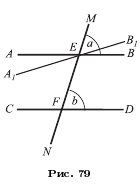
\includegraphics{mppics/ris-79}
\caption{}\label{1938/ris-79}
\end{wrapfigure}

\smallskip
\mbox{\so{Теорема} (обратная теорема, §~\ref{1938/73}).}\\
\textbf{\emph{Если две параллельные прямые}} ($AB$ и $CE$), рис.~\ref{1938/ris-79}) \textbf{\emph{пересечены какой-нибудь прямой}} ($MN$), \textbf{\emph{то:}}


1) \textbf{\emph{соответственные углы равны;}}

2) \textbf{\emph{накрест лежащие углы равны;}}

3) \textbf{\emph{сумма внутренних односторонних углов равна $\bm{180\degree}$;}}

4) \textbf{\emph{сумма внешних односторонних углов равна $\bm{180\degree}$.}}

Докажем, например, что если $AB\z\parallel CD$, то соответственные углы $\alpha$ и $\beta$ равны.


Предположим противное, то есть что эти углы не равны (например, пусть $\alpha \z> \beta$).
Построив $\angle MEB_1 = \beta$, мы получим тогда прямую $A_1B_1$, не сливающуюся с $AB$, и, следовательно, будем иметь две различные прямые, проходящие через точку $E$ и параллельные одной и той же прямой $CD$, именно:
$AB\parallel CD$, согласно условию теоремы, и $A_1B_1\z\parallel CD$ вследствие равенства соответственных углов $\angle MEB_1$ и $ \beta$.
Так как это противоречит аксиоме параллельных линий, то наше предположение, что углы $\alpha$ и $\beta$ не равны, должно быть отброшено;
остаётся принять, что $ \alpha =  \beta$.

 %%%%overfull
Таким же путём можно доказать и остальные заключения теоремы.
Из доказанных выше предложений непосредственно вытекает следующая теорема.

\textbf{\emph{Перпендикуляр к одной из двух параллельных прямых есть также перпендикуляр и к другой.}}

\begin{wrapfigure}[11]{o}{41mm}
\centering
\includegraphics{mppics/ris-80}
\caption{}\label{1938/ris-80}
\end{wrapfigure}

Действительно, если $AB\parallel CD$ (рис.~\ref{1938/ris-80}) и $ME\perp AB$, то, во-первых, $ME$, пересекаясь с $AB$, пересекается и с $CD$ в некоторой точке $F$, во-вторых, соответственные углы $\alpha$ и $\beta$ равны.
Но угол $\alpha$ прямой, значит, и угол $\beta$ прямой, то есть
$ME\perp CD$.

\paragraph{Признаки непараллельности прямых.}
\label{1938/78}
Из двух теорем:
прямой (§~\ref{1938/73}) и ей обратной (§~\ref{1938/77}) можно вывести заключение, что \so{противоположные теоремы} также верны, то есть:

\emph{Если при пересечении двух прямых третьей окажется, что 1) соответственные углы не равны или 2) внутренние накрест лежащие углы \so{не равны} и~т.~д., то прямые \so{не параллельны};
если две прямые \so{не параллельны}, то при пересечении их третьей прямой 1) соответственные углы \so{не равны}, 2) внутренние накрест лежащие углы \so{не равны}} и~т.~д.
Из этих признаков непараллельности (легко доказываемых способом от противного) полезно обратить особое внимание на следующий.

\begin{wrapfigure}[8]{o}{55mm}
\vskip-4mm
\centering
\includegraphics{mppics/ris-81}
\caption{}\label{1938/ris-81}
\end{wrapfigure}

\emph{если сумма внутренних односторонних углов \emph{($\alpha$ и $\beta$, рис.~\ref{1938/ris-81})} не равна $180\degree$, то прямые \emph{($AB$ и $CD$)} при достаточном продолжении пересекаются,} так как если бы эти прямые не пересекались, то они были бы параллельны, и тогда сумма внутренних односторонних углов равнялась бы $180\degree$, что противоречит условию.



Это предложение (дополненное утверждением, что прямые пересекутся по ту сторону от секущей линии, по которой сумма внутренних односторонних углов \so{меньше} $180\degree$) было принято знаменитым греческим геометром Евклидом (жившим в III веке до нашей эры) в его «Началах» геометрии без доказательства как аксиома параллельных линий, и потому оно известно под именем постулата Евклида.
В настоящее время предпочитают принимать за такую аксиому более простое предложение (§~\ref{1938/75}).

Укажем ещё два следующих признака непараллельности, которые понадобятся нам впоследствии:

{

1) \emph{Перпендикуляр \emph{($AB$, рис.~\ref{1938/ris-82})} и наклонная \emph{($CD$)} к одной и той же прямой \emph{($EF$)} пересекаются,} потому что сумма внутренних односторонних углов 1 и 2 не равна $180\degree$.

\begin{figure}[h!]
\begin{minipage}{.48\textwidth}
\centering
\includegraphics{mppics/ris-82}
\end{minipage}\hfill
\begin{minipage}{.48\textwidth}
\centering
\includegraphics{mppics/ris-83}
\end{minipage}

\medskip

\begin{minipage}{.48\textwidth}
\centering
\caption{}\label{1938/ris-82}
\end{minipage}\hfill
\begin{minipage}{.48\textwidth}
\centering
\caption{}\label{1938/ris-83}
\end{minipage}
\vskip-4mm
\end{figure}

2) \emph{Две прямые \emph{($AB$ и $CD$, рис.~\ref{1938/ris-83}),} перпендикулярные к двум пересекающимся прямым \emph{($FE$ и $FG$),} пересекаются.}

 %%%%overfull
Действительно, если предположим противное, то есть
что $AB \parallel CD$, то прямая $FG$, будучи перпендикулярна к одной из параллельных (к $CD$), была бы перпендикулярна и к другой параллельной (к $AB$), и тогда из одной точки $F$ к прямой $AB$ были бы проведены два перпендикуляра:
$FB$ и $FD$, что невозможно.

}

\subsection*{Углы с соответственно параллельными или перпендикулярными сторонами}

\paragraph{}\label{1938/79}
\so{Теорема}.
\textbf{\emph{Если стороны одного угла соответственно параллельны сторонам другого угла, то такие углы или равны, или в сумме составляют два прямых.}}

\begin{wrapfigure}{o}{43mm}
\vskip-0mm
\centering
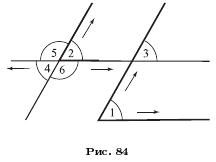
\includegraphics{mppics/ris-84}
\caption{}\label{1938/ris-84}
\end{wrapfigure}

Рассмотрим особо следующие три случая (рис.~\ref{1938/ris-84}).

1) Пусть стороны угла 1 соответственно параллельны сторонам угла 2 и, сверх того, имеют \so{одинаковое направление от вершины} (на чертеже направления указаны стрелками).

Продолжив одну из сторон угла 2 до пересечения с непараллельной ей стороной угла 1, мы получим угол 3, равный и углу 1, и углу 2 (как соответственные при параллельных прямых);
следовательно, $\angle 1 = \angle 2$.

2) Пусть стороны угла 1 соответственно параллельны сторонам угла 4, но имеют противоположное направление от вершины.

Продолжив обе стороны угла 4, мы получим угол 2, который равен углу 1 (по доказанному выше) и углу 4 (как вертикальный ему);
следовательно, $\angle 4 = \angle 1$.

3) Пусть, наконец, стороны угла 1 соответственно параллельны сторонам углов 5 и 6, причём две из этих сторон имеют одинаковое направление, а две другие — противоположное.

Продолжив одну сторону угла 5 или угла 6, мы получим угол 2, который равен (по доказанному) углу 1;
но $\angle 5$ (или $\angle 6) +\angle 2 \z= 180\degree$ (по свойству смежных углов);
следовательно, и $\angle 5$ (или $\angle 6) \z+ \angle 1 \z= 180\degree$.

Таким образом, углы с параллельными сторонами оказываются равными, когда их стороны имеют или одинаковое, или противоположное направление от вершины;
если же это условие не выполнено, то углы составляют в сумме $180\degree$.

\smallskip
\so{Замечание}.
Можно было бы сказать, что углы с параллельными сторонами равны тогда, когда они оба острые или оба тупые;
но бывают случаи, когда по виду углов трудно определить, острые ли они или тупые;
поэтому приходится сравнить направления сторон углов.

\paragraph{}\label{1938/80}
\so{Теорема}.
\textbf{\emph{Если стороны одного угла соответственно перпендикулярны к сторонам другого угла, то такие углы или равны, или в сумме составляют два прямых.}}

Пусть угол $ABC$, обозначенный цифрой 1 (рис.~\ref{1938/ris-85}), есть один из данных углов;
за другой данный угол возьмём какой-нибудь из четырёх углов:
2, 3, 4 или 5, образованных двумя пересекающимися прямыми, из которых одна перпендикулярна к стороне $AB$, а другая — к стороне $BC$ (общая вершина их может находиться в любой точке плоскости).

\begin{wrapfigure}[11]{o}{35mm}
\centering
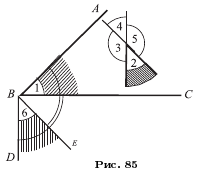
\includegraphics{mppics/ris-85}
\caption{}\label{1938/ris-85}
\end{wrapfigure}

Проведём из вершины угла 1 две вспомогательные прямые:
$BD\perp BC$ и $BE\z\perp BA$.
Образованный ими угол 6 равен углу 1 по следующей причине:
углы $DBC$ и $EBA$ равны, так как оба они прямые;
отняв от каждого из них по одному и тому же углу $EBC$, получим: $\angle 6 = \angle 1$.

Заметим, что стороны вспомогательного угла 6 параллельны пересекающимся прямым, образующим углы 2, 3, 4 и 5 (потому что два перпендикуляра к одной прямой параллельны, §~\ref{1938/71}). 
Следовательно, эти углы или равны углу 6, или составляют с ним в сумме $180\degree$.
Заменив угол 6 равным ему углом 1, получим то, что требовалось доказать.

\subsection*{Сумма углов треугольника и многоугольника}

\paragraph{}\label{1938/81}
\mbox{\so{Теорема}.}
\textbf{\emph{Сумма углов треугольника равна $\bm{180\degree}$.}}

\begin{wrapfigure}[8]{o}{41mm}
\vskip-2mm
\centering
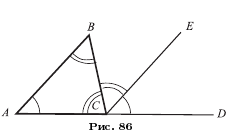
\includegraphics{mppics/ris-86}
\caption{}\label{1938/ris-86}
\end{wrapfigure}

Пусть $ABC$ (рис.~\ref{1938/ris-86}) — какой-нибудь треугольник;
требуется доказать, что сумма углов $A$, $B$ и $C$ равна $180\degree$.
Продолжив сторону $AC$ и проведя $CE\parallel AB$, найдём:
$\angle A = \angle ECD$ (как углы, соответственные при параллельных), $\angle B = \angle BCE$ (как углы, накрест лежащие при параллельных). 
Отсюда
\[\angle A + \angle B+\angle C = \angle ECD + \angle BCE + \angle C =180\degree.\]

\smallskip
\so{Следствия}.
1) \emph{Всякий внешний угол треугольника равен сумме двух внутренних углов, не смежных с ним} (так, $\angle BCD \z= \angle A + \angle B$).

2) \emph{Если два угла одного треугольника соответственно равны двум углам другого, то и третьи углы равны.}

{

\begin{wrapfigure}{o}{38mm}
\centering
\includegraphics{mppics/ris-87}
\caption{}\label{1938/ris-87}
\end{wrapfigure}

3) \emph{Сумма двух острых углов прямоугольного треугольника равна одному прямому углу, то есть $90\degree$.}

4) \emph{В равнобедренном прямоугольном треугольнике каждый острый угол равен $45\degree$.}

5) \emph{В равностороннем треугольнике каждый угол равен $60\degree$.}

6) \emph{Если в прямоугольном треугольнике $ABC$ \emph{(рис.~\ref{1938/ris-87})} один из острых углов \emph{(например $\angle B$)} равен $30\degree$, то лежащий против него катет составляет половину гипотенузы.}

}

Заметив, что в таком треугольнике другой острый угол равен $60\degree$, пристроим к треугольнику $ABC$ другой треугольник $ABD$, равный данному.
Тогда мы получим треугольник $DBC$, у которого каждый угол равен $60\degree$.
Такой равноугольный треугольник должен быть равносторонним (§~\ref{1938/47}), и потому $BC\z=DC$.
Но $AC=\tfrac12DC$, значит, $AC=\tfrac12BC$.

{\sloppy 
Предоставляем самим учащимся доказать обратное предложение:
\emph{если катет равен половине гипотенузы, то противолежащий ему острый угол равен $30\degree$.}

}

\paragraph{}\label{1938/82}
\so{Теорема}.
\textbf{\emph{Сумма углов выпуклого $\bm{n}$-угольника равна $\bm{180\degree\cdot(n-2)}$.}}

Взяв внутри выпуклого $n$-угольника произвольную точку $O$ (рис. \ref{1938/ris-88}), соединим её со всеми вершинами.
Тогда $n$-угольник разобьётся на $n$ треугольников — к каждой его стороне примыкает один треугольник.

\begin{wrapfigure}{o}{30mm}
\centering
\includegraphics{mppics/ris-88}
\caption{}\label{1938/ris-88}
\end{wrapfigure}

Сумма углов каждого треугольника равна $180\degree$ следовательно, сумма углов всех треугольников равна $180\degree\cdot n$.
Эта величина, очевидно, превышает сумму углов $n$-угольника на сумму всех тех углов, которые расположены вокруг точки $O$;
но эта сумма равна $360\degree$;
следовательно, сумма углов $n$-угольника равна:
\[180\degree\cdot n -360\degree = 180\degree\cdot(n - 2).\]

\begin{wrapfigure}{r}{30mm}
\centering
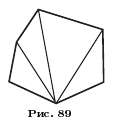
\includegraphics{mppics/ris-89}
\caption{}\label{1938/ris-89}
\end{wrapfigure}


\smallskip
\mbox{\so{Замечание}.}
Эту теорему можно доказать ещё и так:
Из вершины какого-нибудь выпуклого $n$-угольника проведём его диагонали (рис.~\ref{1938/ris-89}).
Тогда $n$-угольник разобьётся на $n-2$ треугольника.
Действительно, если не будем считать двух сторон, образующих угол, из вершины которого проведены диагонали, то на каждую из остальных сторон придётся по одному треугольнику.
Но в каждом треугольнике сумма углов равна $180\degree$.
Значит, сумма углов всех треугольников будет $180\degree\cdot(n-2)$;
но эта сумма и есть сумма всех углов $n$-угольника.

\medskip



\smallskip
\so{Примечание}.
Доказанная теорема верна и для вогнутых многоугольников.
При этом, если внутри $n$-угольника можно найти такую точку, что отрезки, соединяющие её с вершинами $n$-угольника, лежат внутри него, то теорему можно доказать, повторяя дословно те рассуждения, которые мы приводили выше при первом способе доказательства.
Если же такой точки найти нельзя, то следует весь $n$-угольник разбить на треугольники, проведя некоторые его диагонали — можно доказать, что такое разбиение всегда существует и при этом всех треугольников будет $n-2$.
Подсчитав затем сумму углов в каждом из треугольников и сложив эти суммы, получим ту же формулу $180\degree\cdot(n - 2)$.

{

\begin{wrapfigure}{o}{33mm}
\centering
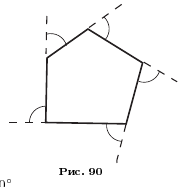
\includegraphics{mppics/ris-90}
\caption{}\label{1938/ris-90}
\end{wrapfigure}

\paragraph{}\label{1938/83}
\mbox{\so{Теорема}.}
\textbf{\emph{Если из вершины каждого угла выпуклого многоугольника проведём продолжение одной из сторон этого угла, то сумма всех образовавшихся при этом внешних углов многоугольника равна $\bm{360\degree}$}} (независимо от числа сторон многоугольника).

Каждый из таких внешних углов (рис.~\ref{1938/ris-90}) составляет дополнение до $180\degree$ к смежному с ним внутреннему углу многоугольника.

Следовательно, если к сумме всех внутренних углов $n$-угольника прибавим сумму всех внешних углов, то получим $180\degree\cdot n$;
но сумма внутренних углов, как мы видели, равна $180\degree\cdot (n - 2)$;
следовательно, сумма внешних углов равна разности:
\begin{align*}
&180\degree\cdot n-180\degree\cdot (n - 2)=
\\
=~&180\degree\cdot n-180\degree\cdot n+360\degree=
\\
=~&360\degree.
\end{align*}

}

\subsection*{Центральная симметрия}

\paragraph{}\label{1938/84}
В §~\ref{1938/37} был рассмотрен случай симметричного расположения двух равных фигур относительно прямой.
Выведенные выше свойства параллельных прямых позволяют изучить ещё один замечательный вид расположения двух равных фигур, или двух равных отрезков, или двух точек по отношению к некоторой точке на плоскости.

\begin{wrapfigure}{o}{25mm}
\vskip-2mm
\centering
\includegraphics{mppics/ris-91}
\caption{}\label{1938/ris-91}
\end{wrapfigure}

\textbf{Если две какие-либо точки $\bm{A}$ и $\bm{A'}$} (рис.~\ref{1938/ris-91}) \textbf{расположены на одной прямой с точкой $\bm{O}$ по разные стороны от неё и на одинаковом от неё расстоянии} ($OA=OA'$), \textbf{то такие точки называются симметричными относительно точки} ($O$).

Чтобы построить точку, симметричную с данной точкой $A$ относительно другой данной точки $O$, следует соединить точки $A$ и $O$ прямой, продолжить эту прямую за точку $O$ и отложить на ней от точки $O$ отрезок $OA'$, равный $OA$, таким образом, чтобы точки $A$ и $A'$ были расположены по разные стороны относительно точки $O$.
Точка $A'$ будет искомой.

\paragraph{}\label{1938/85}
\so{Теорема}.
\textbf{\emph{Если для двух точек $\bm{A}$ и $\bm{B}$ какой-либо прямой $\bm{AB}$ построить симметричные им точки $\bm{A'}$ и $\bm{B'}$ относительно некоторой точки $\bm{O}$ то:}}

\begin{wrapfigure}{r}{35mm}
\centering
\includegraphics{mppics/ris-92}
\caption{}\label{1938/ris-92}
\end{wrapfigure}


1) \textbf{\emph{Прямая, соединяющая точки $\bm{A'}$ и $\bm{B'}$, будет параллельна данной прямой $\bm{AB}$, причём отрезок $\bm{AB}$ равен отрезку $\bm{A'B'}$.}}

2) \textbf{\emph{Каждой точке данной прямой $\bm{AB}$ соответствует симметричная ей точка на построенной прямой $\bm{A'B'}$.}}

\smallskip

1) Треугольники $AOB$ и $A'OB'$ равны (рис.~\ref{1938/ris-92}), потому что у них $AO=A'O$ и $BD\z=B'O$ (по построению), $\angle AOB=\angle A'OB''$ (как вертикальные углы).
Из равенства этих треугольников следует:
$AB=A'B'$ и $\angle OAB \z= \angle OA'B'$;
значит, $AB\parallel A'B'$ (§~\ref{1938/73}, 2-й случай).

2) Возьмём на прямой $AB$ какую-либо точку $D$ (рис.~\ref{1938/ris-92}).
Рассмотрим прямую, соединяющую точку $D$ с точкой $O$.
Эта прямая пересечёт прямую $A'B'$ в некоторой точке $D'$.
Треугольники $AOD$ и $A'OD'$ равны, потому что у них $AO\z=A'O$, $\angle 1 = \angle 2$ (как накрест лежащие при параллельных прямых) и $\angle 3 = \angle 4$ (как вертикальные).
Из равенства этих треугольников следует:
$OD = OD'$.
Значит, точки $D$ и $D'$ симметричны относительно точки $O$.


\paragraph{Симметричные фигуры.}\label{1938/86}
\textbf{\emph{Две фигуры называются симметричными относительно данной точки $\bm{O}$, если каждой точке одной фигуры соответствует симметричная ей точка другой фигуры.}} 

Точка $O$ называется \rindex{центр симметрии}\textbf{центром симметрии} данных фигур.
Сама симметрия называется \rindex{центральная симметрия}\textbf{центральной} в отличие от осевой, с которой мы уже встречались раньше (§~\ref{1938/37}).
Если каждой точке данной фигуры соответствует симметричная ей точка той же самой фигуры (относительно некоторого центра), то говорят, что данная фигура имеет центр симметрии.
Примером такой фигуры служит окружность.
Центром её симметрии является её центр.

\textbf{Каждую фигуру можно совместить с фигурой, ей симметричной, путём вращения её вокруг центра симметрии.}

В самом деле, возьмём, например, два треугольника $ABC$ и $A'B'C'$ (рис.~\ref{1938/ris-93}), симметричные относительно некоторого центра $O$.

Всю фигуру $OABC$, не отрывая от плоскости, будем вращать вокруг точки $O$ как вокруг центра до тех пор, пока прямая $OA$ не пойдёт по $OA'$.

Так как $\angle 1 = \angle 2$ и $\angle 3 = \angle 4$, то прямая $OB$ пойдёт по $OB'$, а прямая $OC$ по $OC'$.

\begin{wrapfigure}{o}{45mm}
\vskip-2mm
\centering
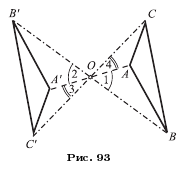
\includegraphics{mppics/ris-93}
\caption{}\label{1938/ris-93}
\end{wrapfigure}

Так как $OA = OA'$, $OB=OB'$, $OC\z=OC'$, то точка $A$ совпадёт с $A'$, точка $B$ с $B'$ и точка $C$ с $C'$.
Таким образом, треугольник $ABC$ совместится с треугольником $A'B'C'$.

Очевидно, что при таком повороте каждая прямая $OA$, $OB$, $OC$, а также каждая сторона треугольника $ABC$ повернётся на $180\degree$.
Если фигура имеет центр симметрии, то после поворота её вокруг центра симметрии на $180\degree$ эта фигура совместится сама с собой.

\begin{figure}[h!]
\begin{minipage}{.68\textwidth}
\centering
\begin{lpic}[t(1 mm),b(1 mm),r(0 mm),l(0 mm)]{jpg/Manning_propeller(.8)}
\lbl[b]{54,19;$O$}
\end{lpic}
\end{minipage}
\hfill
\begin{minipage}{.28\textwidth}
\centering
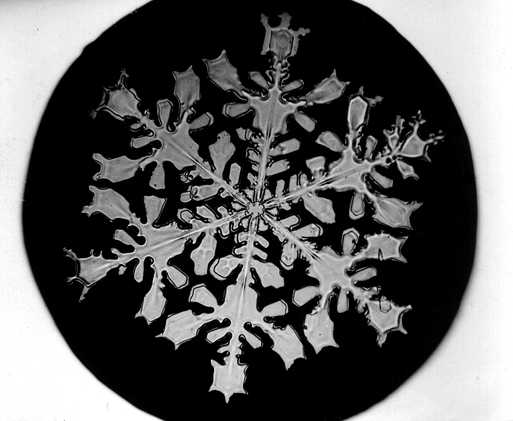
\includegraphics[scale=.19]{jpg/Bentley_Snowflake18}
\end{minipage}

\medskip

\begin{minipage}{.68\textwidth}
\centering
\caption{}\label{1938/ris-94}
\end{minipage}
\hfill
\begin{minipage}{.28\textwidth}
\centering
\caption{}\label{1938/ris-95}
\end{minipage}
\vskip-4mm
\end{figure}

\so{Замечание}.
При вращении, которое мы произвели для совмещения треугольников $ABC$ и $A'B'C'$, треугольник $ABC$ скользил по плоскости.
Таким образом, фигуры, симметричные относительно центра, можно совместить, не выводя их из плоскости.
Этим центральная симметрия существенно отличается от осевой (§~\ref{1938/37}), где для совмещения симметричных фигур необходимо было одну из них перевернуть другой стороной.

Центральная симметрия фигур, так же как и осевая, весьма часто встречается в природе и в обыденной жизни.
На рис.~\ref{1938/ris-94} приведено изображение пропеллера самолёта.
Оно имеет центром симметрии точку $O$.
На рис.~\ref{1938/ris-95} дано изображение снежинки, оно также обладает центром симметрии.
